\documentclass[]{article}
\usepackage[numbers,sort,compress]{natbib}

\usepackage{url}
\usepackage{graphicx}
\usepackage{color}
\usepackage{setspace}
\usepackage{lineno}

\usepackage{authblk}
\title{Demographic inference using the SFS with \moments and \demes}
\author[1]{Nick Collier}
\author[1,*]{Aaron P. Ragsdale}
\affil[1]{Department of Integrative Biology, University of Wisconsin--Madison}
\affil[*]{apragsdale@wisc.edu}
\affil[ ]{ORCID IDs: 0009-0005-0385-9798 (NC), 0000-0003-0715-3432 (APR)}

\usepackage[margin=1in, headheight=15pt, headsep=10pt]{geometry}
\usepackage{fancyhdr}
\pagestyle{fancy}
\lhead{N Collier and AP Ragsdale}
\rhead{Demographic inference with \moments and \demes}

% use minted for python and YAML code
\usepackage{minted}

% local definitions
\usepackage{xspace}
\newcommand{\aprcomment}[1]{{\textcolor{blue}{APR: #1}}}
\newcommand{\reviewercomment}[1]{{\textcolor{red}{REVIEWER: #1}}}
\newcommand{\moments}{\texttt{moments}\xspace}
\newcommand{\demes}{\texttt{demes}\xspace}
\newcommand{\demesdraw}{\texttt{demesdraw}\xspace}
\newcommand{\msprime}{\texttt{msprime}\xspace}
\newcommand{\momi}{\texttt{momi}\xspace}
\newcommand{\fwdpy}{\texttt{fwdpy11}\xspace}
\newcommand{\tskit}{\texttt{tskit}\xspace}

\begin{document}
\linenumbers
\doublespacing

\maketitle

\begin{abstract}

    The site frequency spectrum (SFS) describes the distribution of allele
    frequencies in one or more populations and sees wide use in evolutionary
    inference. Here we show how to use \moments, a Python library for working
    with the SFS and other measures of genetic diversity, and \demes, a
    standard format for parameterizing population models, to infer demographic
    history. Following an introduction to SFS inference, we illustrate the
    general usage of \moments and its \demes interface, and then show two
    specific examples, using both simulated and human genetic data. We conclude
    with caveats and considerations regarding the \moments library and SFS
    inference more broadly.

\end{abstract}

\emph{Keywords:} Demographic inference, site frequency spectrum, \aprcomment{any others?}

% TODO:
% - orcid numbers if any - done
% - interline double, also for references - done
% - line numbers - done
% - keywords - done
% - running head - done
% - Figures in separate files (named Figure 1, Figure2, etc) for the final submission, legends listed at the end of the chapter. - done

\section*{Introduction}

The genetic composition of a sample of individuals is shaped by their genome
biology and evolutionary history. Variation resulting from this history can be
fully represented by the ancestral relationships among samples at each locus in
the genome and how those gene-genealogical relationships change along a
chromosome due to recombination (that is, by information stored in the
Ancestral Recombination Graph; see chapters 1, 8 and 11, and
\cite{nielsen2025inference}). However, the ARG can be large and unwieldy, and
methods for reconstructing history directly from the ARG, while showing promise
(e.g., \cite{yc2022evaluation, fan2023likelihood, brandt2024promise}), are in
their infancy and so far limited in application and scalability. Instead,
evolutionary inference using informative summaries of genetic variation remains
a tractable and powerful alternative for learning parameters of population
history, natural selection and genome biology.

One such summary that has seen wide use is the site frequency spectrum (SFS),
which stores the counts (observed or expected) of alleles carried by a given
number of genomes in a set of samples. Like any summary of the data, the SFS
discards some information stored in the ARG -- in this case, loci are treated
independently so that haplotypic information is lost. Even so, the relative
densities of allele frequencies and the overall scale of the SFS are both
sensitive to demographic and non-demographic processes.

This chapter focuses on multi-population demographic inference from the SFS
using \moments \cite{jouganous2017inferring}.

Briefly, \moments \ldots. 

\reviewercomment{A short paragraph
    briefly describing the principle of the moments methods would be great. How
    does it differ from other sfs based methods? Just for the readers to get an
idea, then directing them to the relevent literature for more details.}


Past population processes, including changes in population size, splits, gene flow
and population structure, impact the SFS in predictable ways. A population size
expansion (or contraction) leads to a relative excess (or deficit) of
low-frequency variants, for example, and commonly used statistics measuring
population divergence, such as $F_{ST}$, are themselves summaries of the SFS.
Thus, the development of methods to learn demographic history from the SFS came
soon after the publication of whole-genome sequencing from multiple individuals
\cite{marth2004allele, williamson2005simultaneous}. More recent methodological
advances allow for increased sample sizes and numbers of populations, providing
a rich ecosystem of software for SFS-based demographic inference
\cite{gutenkunst2009inferring, excoffier2011fastsimcoal,
    gravel2011demographic, jouganous2017inferring, ragsdale2018genomic,
kamm2020efficiently, dilber2024faster}. We return to this in the final section:
Considerations and Caveats.

Other evolutionary mechanisms are known to affect allele frequency dynamics and
the SFS. This presents a challenge for demographic inference, as the observed
SFS may be distorted by non-demographic processes. However, this also presents
an opportunity to learn about different evolutionary processes, if demographic
history can be controlled for. The SFS has been used to infer the distribution
of fitness effects of new mutations, primarily for nonsynonymous variation in
coding regions (e.g., \cite{eyre2006distribution, boyko2008assessing,
kim2017inference}); to scan for historical selective sweeps
(e.g., \cite{kim2002detecting, nielsen2005genomic}); and to understand how
selection on quantitative traits impacts the genetic architecture underlying
those traits (e.g., \cite{patel2024conditional, ragsdale2024archaic}). The SFS
has also been used to infer relative mutation rates and how they have changed
over time \cite{dewitt2021nonparametric}. Each of these analyses typically
requires partitioning the data in some way -- by functional annotation,
mutation context, local recombination rate, etc -- so that comparisons can be
made across SFS from different classes of mutations.

\subsection*{Obtaining and installing the software}

\moments is available through \texttt{pypi} as \texttt{moments-popgen} (using
\texttt{pip install moments-popgen}). Source code can be downloaded from
\url{https://github.com/MomentsLD/moments}, and  documentation is hosted at
\url{https://momentsld.github.io/moments/}. The detailed online examples
accompanying this chapter can be found at
\url{https://github.com/StatisticalPopulationGenomics-2ndEd/moments/}, which uses
\moments version 1.4 and \demes version 0.2.

\subsection*{Interfacing \moments with \demes}

Specifying demographic models requires defining populations (or ``demes'') and
their relationships via splits and gene flow. \demes provides a standardized
and accessible format for defining demographic models \cite{gower2022demes},
and has been adopted by widely used software for population genetics simulation
and inference (including \msprime \cite{baumdicker2022efficient}, \momi
\cite{dilber2024faster}, \fwdpy \cite{thornton2019polygenic}, and
\texttt{GADMA} \cite{noskova2023gadma2}). \demes encourages interoperability
and reuse of code across software, ease of model implementation and reduction
of errors.

Demographic models are specified in YAML format (see \cite{gower2022demes} and
the associated documentation). To illustrate, the two-population
split-with-migration model depicted in Figure~\ref{fig:im}A is specified as
below:

\singlespacing
\begin{minted}[gobble=4, frame=single,]{yaml}
    description: split-with-migration model, loosely based on example 2
    generation_time: 29
    time_units: years
    demes:
    - name: ancestral
      epochs:
      - {start_size: 15000, end_time: 300000}
      - {start_size: 25000, end_time: 75000}
    - name: popA
      ancestors: [ancestral]
      epochs:
      - {start_size: 30000}
    - name: popB
      ancestors: [ancestral]
      epochs:
      - {start_size: 1200, end_size: 14000}
    migrations:
    - demes: [popA, popB]
      rate: 5e-5
\end{minted}
\doublespacing

In \moments, a \demes-specified demographic model can be directly used to
compute expectations for either the SFS or multi-population LD statistics
\cite{ragsdale2019models, ragsdale2020unbiased}. For the SFS, we simply need
to load the demographic model using \demes and then specify the number of
haploid samples to draw and from which populations.
\begin{minted}[gobble=4, frame=single]{python}
    import demes, moments
    g = demes.load('model.yaml')
    samples = {'popA': 60, 'popB': 60}
    fs = moments.Demes.SFS(g, samples=samples)
\end{minted}
Here, we have not specified a mutation rate. The default behavior sets $u=1$,
so that $\theta = 4N_eu=4N_e$, where $N_e$ is the ancestral population's
initial size. With a known mutation rate, the SFS will be properly scaled by
passing the mutation rate as a keyword argument: \texttt{moments.Demes.SFS(g,
samples=samples, u=u)}. This is equivalent to scaling the output SFS above by
multiplying by \texttt{u}, as \texttt{u*fs}.

\section*{Examples: inference in \moments using \demes}

Below, we show two examples of multi-population demographic inference using the
joint SFS. The first example simulates data with known demographic parameters,
which we try to reinfer using the both the original model and simpler
misspecified models. In the second example, we infer a relatively simple
human-Neanderthal history using data from two human populations and a
high-coverage ancient sample from the Neanderthal lineage. For both of these
examples, we briefly describe data processing and inference setup, emphasizing
the high-level components of the analyses. For detailed information about each
example, including managing data, specifying models, performing inference,
computing confidence intervals and visualizing fits, we refer readers to the
accompanying GitHub repository
(\url{https://github.com/StatisticalPopulationGenomics-2ndEd/moments}), which
is maintained with up-to-date versioning.

\reviewercomment{Would it be possible to include some information regarding possible local optima? Do you recommend starting from different initial conditions?}

In order to optimize parameters in a \demes model, we need a way to specify
which parameters should be fit. For this, we use a separate YAML-formatted file
to define \texttt{parameters}, each of which points to desired value(s) in the
demographic model and for which lower and upper bounds may be set. This file
also specifies any relative \texttt{constraints} between pairs of parameters,
to ensure the optimization routine only explores valid model space. Below, we
have included a truncated parameters file -- the full example is available on
GitHub (URL above).

\singlespacing
\begin{minted}[gobble=4, frame=single]{YAML}
    parameters:
    - name: T0
      values:
      - demes:
          ancestral:
            epochs:
              0: end_time
      lower_bound: 0
      upper_bound: 2e5
    - name: T1
      values:
      - demes:
          ancestral:
            epochs:
              1: end_time
      lower_bound: 0
      upper_bound: 1e6
    - name: Ne
      values:
      - demes:
          ancestral:
            epochs:
              0: start_size
      lower_bound: 1e2
      upper_bound: 1e6
    ...
    constraints:
    - params: [T0, T1]
      constraint: greater_than
\end{minted}
\doublespacing

Taking the demographic model, parameters file, and observed SFS together, we
can perform inference using the \texttt{moments.Demes.Inference.optimize()}
function. The initial parameter guesses are given by the input demographic
model, which may be perturbed using a keyword argument. Any value in the
demographic model that is not specified in the parameters file will remain
unchanged, and is therefore treated as a fixed parameter. Here, we also assume
we have an estimate for the total mutation rate, $U$.

\singlespacing
\begin{minted}[gobble=4, frame=single]{python}
    import moments 

    data = moments.Spectrum.from_file('data.fs')
    U = 1e-8 * 5e8  # per-base mutation rate times the total length

    model_file = 'model.yaml'
    params_file = 'params.yaml'
    output = 'model.fit.yaml'

    ret = moments.Demes.Inference.optimize(
        model_file, params_file, data,
        perturb=1, uL=U, output=output
    )
\end{minted}
\doublespacing

Confidence intervals may also be computed using
\texttt{moments.Demes.Inference.uncerts()}, once a (locally) optimal model has
been found. The following will emit a tab-separated file containing parameter
names, best-fit values and estimated standard errors.

\singlespacing
\begin{minted}[gobble=4, frame=single]{python}
    log_file = 'log.txt'

    uncerts = moments.Demes.Inference.uncerts(
        output, params_file, data,
        uL=U, output=log_file
    )
\end{minted}
\doublespacing

Uncertainties may be computed using either the Fisher Information Matrix, which
tends to underestimate confidence intervals due to nonindependence of linked
sites, or using the Godambe Information Matrix, which uses a set of
bootstrapped datasets to correct for this nonindependence in the data
\cite{coffman2016computationally}. Example 1 in the associated GitHub
repository demonstrates this using a simulated dataset.

\subsection*{Example 1: Inferring parameters in a simulated split-with-migration model}

Using the split-with-migration model defined above (illustrated in
Figure~\ref{fig:im}A), we simulated data for 30 diploid individuals from both
populations using \msprime \cite{baumdicker2022efficient}. These simulations
consided of 500 regions, each of length 1 Mb, with per-base recombination and
mutation rates of $10^{-8}$. The joint SFS was computed using \tskit's
\texttt{ts.allele\_frequency\_spectrum()} function separately on each replicate
region and summing across regions to find the total SFS across 500 Mb of data
(Figure~\ref{fig:im}B--D).

We fit three demographic models to the simulated data. In addition to
reinferring the parameters from the simulated model, we fit two simpler models
to the same data. These had fewer parameters, both omitting the size change
deeper in time in the ancestral population. This is meant to crudely mimic the
scenario that we often face, in which the true history is more complicated than
the parameterized model. It also highlights biases in inferences that can arise
when features of the true history are not included.

When fitting the two misspecified models that do not allow for size changes in
the ancestral population, this split time is inferred to be substantially
deeper in the past than the true split time. This effect, as demonstrated in
\cite{momigliano2021biases}, is due to the decreased coalescence rate within
the ancestral population between the time of the expansion and divergence of
the descendent populations. These two misspecified models
(Figure~\ref{fig:im}H,I) also provide a worse fit to the data, as seen by the
lower log-likelihoods and the large residuals between model predictions and
data (Figure~\ref{fig:im}E-G).

\subsection*{Example 2: Inferring human-Neanderthal demographic parameters}

This example uses publicly available data to infer a demographic model for two
human groups (a northern European and western African population) and a
Neanderthal individual. As shown below, even with just a single sample from the
Neanderthal lineage, we are able to recover key parameters such as the
human-Neanderthal divergence and introgression proportion.

We obtained modern human genome sequences from a recent resequencing of the 
1000 Genomes Project cohort \cite{byrska2022high}, and used the high-coverage 
sequence of the Vindija Neandertal from \cite{prufer2017high}. 
From the 1000 Genomes cohort we took 85 MSL (Mende from Sierre Leone) and 91 
GBR (British from England and Scotland) sequences as our modern human samples.  
We filtered out sites that lay outside the 1000 Genomes `strict' mask, 
were not genotyped in the high-coverage archaic genome sequences, 
that lacked high-confidence ancestral state assignments, or fell within 10 kb of 
exonic or promoter regions. This left us with approximately 960 Mb of 
well-characterized and putatively neutrally-evolving sequence.
We estimated the genome-wide SFS using built-in \moments parsing functions.
Details concerning data processing (including our liftover of the Vindija 
sequence to a more recent genome build) can be found in the linked GitHub 
repository.

The model that we wished to fit is relatively simple but still has many 
parameters ($11$ in the example we present), so we constructed it in stages by 
first fitting simpler one-- and two--population models.
Throughout, we used $u=1.5\times 10^{-8}$ as an estimate of the mutation rate per 
generation and 29 years as the average generation time. When the goal is to infer
a complex demographic history involving multiple populations, we typically start
simple, with subsets of the full data, and sequentially add complexity.
Here, we began by fitting 
one-population models with ancestral and recent size changes for MSL and GBR.
For the MSL model, we allowed three epochs with constant effective size in each 
epoch. We attributed to GBR a sharp contraction $\sim$60 kya followed by 
exponential growth to represent the out-of-Africa bottleneck and subsequent 
rapid expansion. YAML files representing the models and parameters in this 
section can be found in the linked GitHub repository.

\reviewercomment{maybe it would be helpful to also include the likelihood (or AIC?) of each step to show how it changes with the addition of further parameters, and how it can be used to inform the models design}
\aprcomment{this suggestion would only make sense for models fit to the same data SFS, but it could be done to compare the fit without vs. with the Neanderthal pulse. Maybe we could demonstrate the likelihood ratio test, if it works? what do you think, Nick?}

We next stitched these one-population models together and refitted the 
resulting demographic model to get a two-population model 
that included continuous symmetric 
migration between MSL and GBR and an ancestral size expansion. Following this,
we added a Neandertal branch and fitted the 
Neandertal-modern human divergence time, Neandertal effective size, and the 
Neandertal-to-GBR admixture proportion. We also fitted the divergence time 
between the sampled Vindija Neandertal lineage and the Neandertal lineage which 
admixed with modern non-African humans. Finding that this parameter tended to 
converge to its lower bound (imposed by the estimated time of death of the 
Vindija Neandertal, ~55 kya), we fixed it to a value supported by literature 
(90 kya, \cite{prufer2017high}) in a second round of optimization.
Rather than fitting it, we fixed the time of the Neandertal-GBR pulse to 50 kya.
Fixing parameters for which good estimates are available in the literature 
(see, e.g., \cite{sumer2025earliest}) may be reasonable in the first stages of 
model optimization, and we expected this value to be especially difficult to fit 
due to the small pulse proportion and Neandertal sample size. In the second 
round of optimization on the three-population model, we refit all parameters 
aside from the two event times mentioned above to refine the estimates. 

After this refitting step, we were left with parameters in good agreement with 
prior authors, with a Neandertal-modern human divergence time of 547 kya, 
MSL-GBR split time of 77 kya, and Neandertal-GBR pulse proportion of 2.7 
percent. We observe some large, systematic residuals in our best-fit model 
(Figure~\ref{fig:humans}G-I), suggesting model misspecification that could be
improved through further exploration of model space.


\section*{Considerations and caveats}\label{sec:conclusions}

The site frequency spectrum is just one of many options for inferring
evolutionary parameters from genetic data. It is straightforward to compute
from data, and there are many methods for predicting the SFS, making it an
appealing framework for demographic inference. As shown here in two examples,
we have incorporated the \demes format for specifying demographic models in
\moments to easily compute the SFS and perform demographic inference, including
computing uncertainties.

\moments is limited in the size of the dataset that it can consider. Sample
sizes can be large (in the hundreds), especially when considering models with
one or few populations, but will encounter memory issues when sample sizes are
extreme or as the number of populations grows. We are limited to a maximum of
five populations existing at any one time, including ancient samples. Other
SFS-based methods, such as \momi \cite{kamm2020efficiently, dilber2024faster},
can include additional populations, typically with smaller sample sizes.

\reviewercomment{Mirroring my comments in the introduction, I would suggest to add a few sentences to highlight how moments differ from other approaches, in terms of caveats and advantages. No need to go in details, just the take-home message and references for further details.}

When inferring models with multiple populations, especially four or more, both
the numbers of parameters and the space of plausible model topologies can grow
rapidly. It can therefore become challenging for the optimization routines to
find optima in parameter space, and overparameterization can become a problem.
One hint that models are overparameterized (or models misspecified) is runaway
behavior of parameter values, in which they converge to unreasonably small or
large values (or approach the imposed bounds). Starting with simple
parameterizations and sequentially adding complexity helps to alleviate this
issue. The challenge of large model space is more difficult to address, and
must be addressed through building and testing a wide range of plausible model
topologies. While time-consuming, a broad exploration of model space,
especially when considering many populations, is crucial for evaluating
robustness of particular features of inferred history.

Finally, natural selection distorts allele frequencies not only at sites
directly under selection, but also in linked regions of the genome through
background selection. This can have a sizeable impact on the SFS and lead to
biases in demographic inference \cite{ewing2016consequences, johri2021impact}.
In gene-sparse species, such as primates, considering data from regions away
from functionally constrained elements is feasible, as we did in example 2
here.  Alternatively, the genome may be partitioned by $B$-value (a
measure of the local strength of background
selection, \cite{mcvicker2009widespread}) and regions experiencing low levels of
background selection may be used (for an example,
see \cite{medina2023demographic}). In some species with gene-dense genomes, such as
\emph{Drosophila} species, this may be infeasible, and interspersed putatively
neutral variation must be used, such synonymous variation or short introns,
which will still experience background selection. The appropriate strategy will
depend on the genome architecture of the species and genomic resources
available.


\bibliographystyle{unsrt}
\bibliography{paper}

\clearpage

\begin{figure}
    %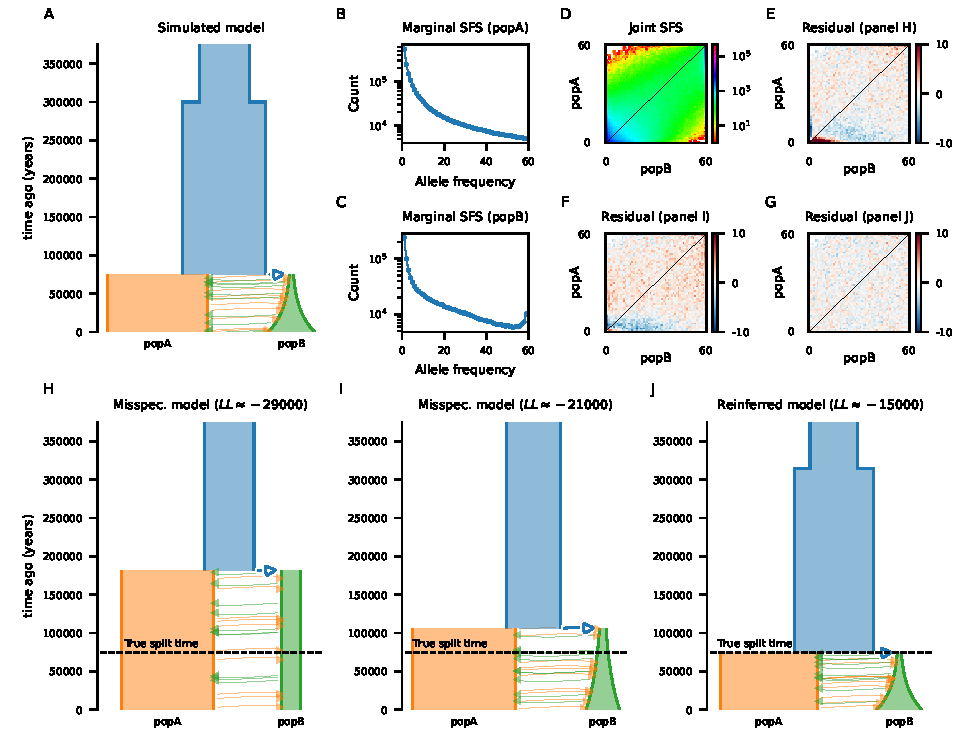
\includegraphics{../example1/fig1.pdf}
    \caption{
        Inference using simulated data. (A) The true demographic model,
        including an expansion in the ancestral population and symmetric
        migration between the descendent populations. (B--D) The simulated
        data, showing both marginal and the joint SFS. (E--G) Residuals
        between the data SFS (in D) and the predicted SFS from the inferred
        demographic models in (H--J), resp.  The two misspecified models (H and
        I) provide worse fits to the data and both overestimate the split time
        due to disallowing any size change in the ancestral population.
        \reviewercomment{it might be good to label the colorbars for the joint spectra as 'allele frequency' for people that are unfamiliar with what those plots are showing}
    }
    \label{fig:im}
\end{figure}

\begin{figure}
    %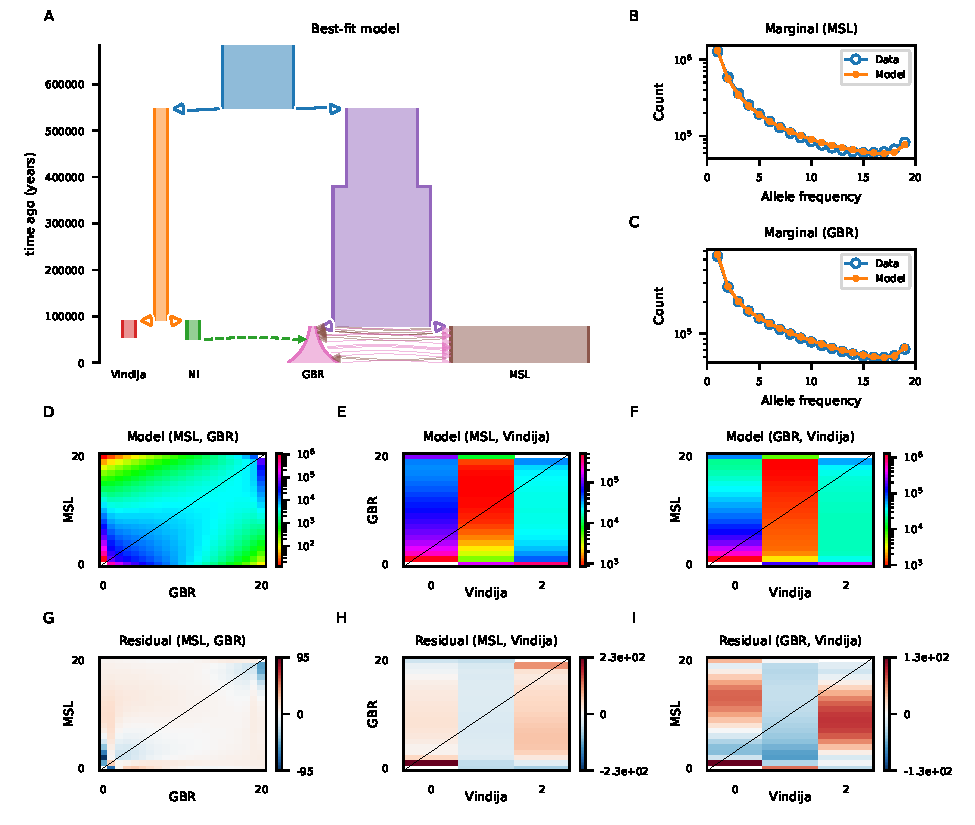
\includegraphics{../example2/fig2.pdf}
    \caption{
        Inference using human and Neanderthal data.
        (A) The best-fit model including the Vindija Neanderthal and two human
        populations.
        (B, C) Marginal SFS fits between the model and empirical data are shown
        for MSL and GBR.
        (D--I) Marginal two-way spectra predicted by the model and their residuals 
        against the data are plotted for the three pairs of populations MSL, GBR 
        (D and G), MSL, Vindija (E and H), and GBR, Vindija (F, I).
    }
    \label{fig:humans}
\end{figure}



\end{document}
